

\begin{figure}[tb]
  \begin{center}
    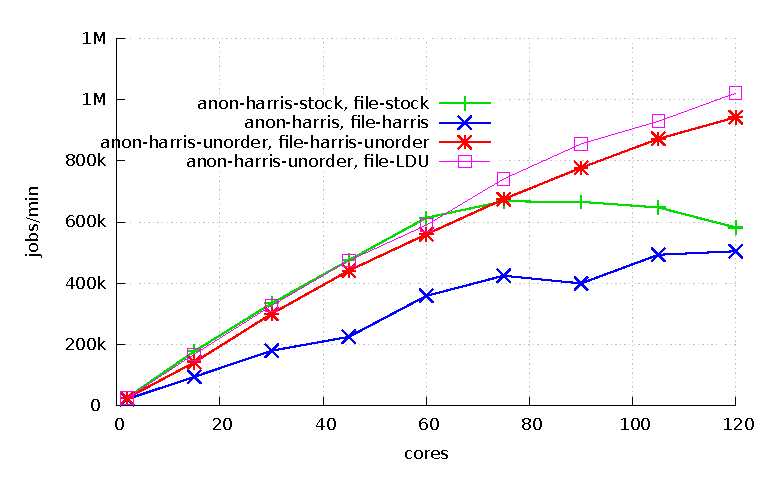
\includegraphics[scale=0.65]{graph/aim7.eps}
  \end{center}
  \caption{Scalability of AIM7 multiuser for different method.  The combination
  \deferu with unordered harris list scale well;in contrast, up to 60 core, the
  stock Linux scale linearly, then it  flattens out.}
  \label{fig:aim7}
\end{figure}

\section{Evaluation}



\begin{figure*}[tb]
    \centering
    \begin{subfigure}[b]{0.33\textwidth}
        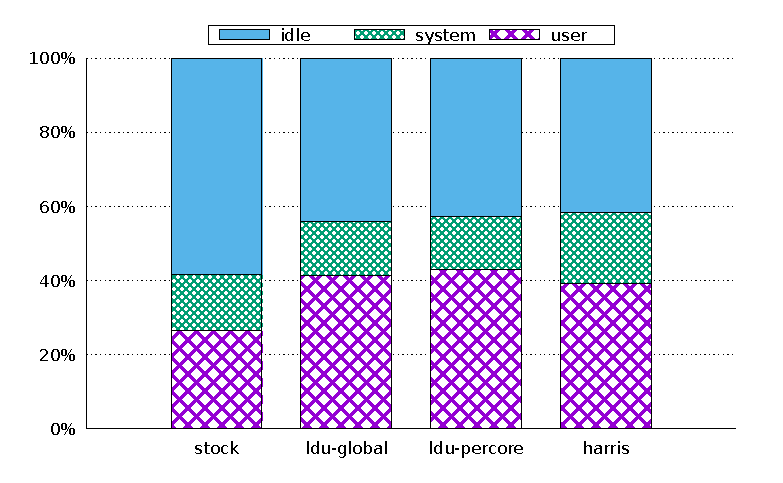
\includegraphics[height=1.3in]{graph/aim7_cpuutils.eps}
        \caption{AIM7 - 120core}
    \end{subfigure}%
    \begin{subfigure}[b]{0.33\textwidth}
        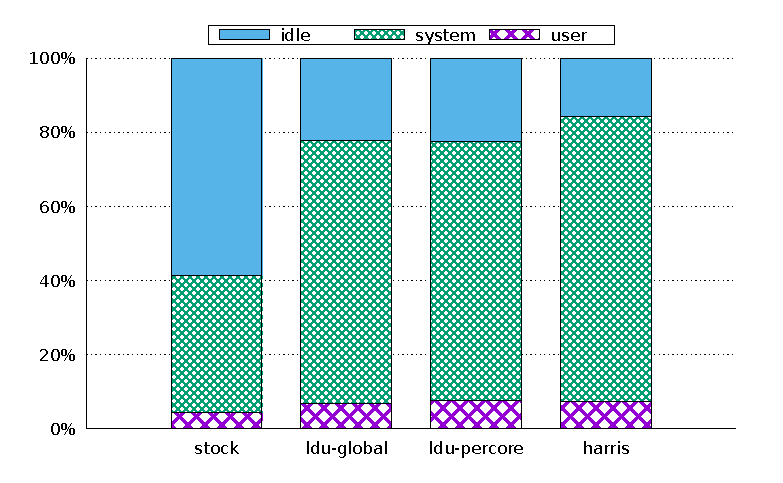
\includegraphics[height=1.3in]{graph/exim_cpuutils.eps}
        \caption{Exim - 120core}
    \end{subfigure}
    \begin{subfigure}[b]{0.33\textwidth}
        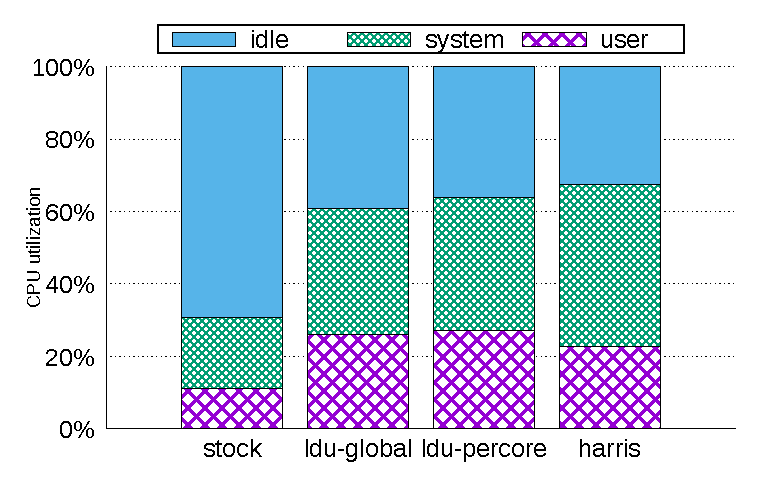
\includegraphics[height=1.3in]{graph/lmbench_cpuutils.eps}
        \caption{Lmbench - 120core}
    \end{subfigure}
        \centering
    \caption{Read-write ratio from 50:50 to 1:99 percent}
    
\end{figure*}


%$$$$$$$$$$$$$$$$$$$$$$$$$$$$$$$$$$$$$$$$$$$$$$$$$$$$$$$$$$$$$$$$$$$$$$$$$$$$$$$$
%Paragraph 1: 무엇을 평가 했는지에 대한 설명 
%$$$$$$$$$$$$$$$$$$$$$$$$$$$$$$$$$$$$$$$$$$$$$$$$$$$$$$$$$$$$$$$$$$$$$$$$$$$$$$$$

\subsection{Experimental setup}

%$$$$$$$$$$$$$$$$$$$$$$$$$$$$$$$$$$$$$$$$$$$$$$$$$$$$$$$$$$$$$$$$$$$$$$$$$$$$$$$$
%Paragraph 3: 운영체제 및 커널 버전 설명
%$$$$$$$$$$$$$$$$$$$$$$$$$$$$$$$$$$$$$$$$$$$$$$$$$$$$$$$$$$$$$$$$$$$$$$$$$$$$$$$$
We ran the three benchmarks on Linux 4.5.0 rc6 with stock Linux. 
All experiments were performed on a 120 core machine with 8-socket, 15-core
Intel E7-8870 chips equipped with 792 GB DDR3 DRAM.

%$$$$$$$$$$$$$$$$$$$$$$$$$$$$$$$$$$$$$$$$$$$$$$$$$$$$$$$$$$$$$$$$$$$$$$$$$$$$$$$$
%Paragraph 1: 벤치 마크 대한 설명
%$$$$$$$$$$$$$$$$$$$$$$$$$$$$$$$$$$$$$$$$$$$$$$$$$$$$$$$$$$$$$$$$$$$$$$$$$$$$$$$$
Fork-intensive applications benefit from the designs described in this
research, so we use well-known three fork-intensive benchmarks:AIM7, a Linux
scalability benchmark;Exim, an email server in MOSBENCH;and Lmbench, a micro
benchmark.
The workloads exhibit the high lock contentions because of the reverse mapping.
Moreover, the AIM7 benchmark is widely used in the Linux community not only for
testing the Linux kernel but also for improving the scalability. 
The Exim is a real world application, but it has scalability bottlenecks caused
by the Linux fork.
Finally, in order to only focus on the fork performance and scalability, we
selected the Lmbench.

%$$$$$$$$$$$$$$$$$$$$$$$$$$$$$$$$$$$$$$$$$$$$$$$$$$$$$$$$$$$$$$$$$$$$$$$$$$$$$$$$
%Paragraph 2-1: Harris Lock free list 구현 내용에 대한 설명 
%$$$$$$$$$$$$$$$$$$$$$$$$$$$$$$$$$$$$$$$$$$$$$$$$$$$$$$$$$$$$$$$$$$$$$$$$$$$$$$$$
In order to compare our \deferu implementation to a concurrent non-blocking
Harris linked list ~\cite{Harris2001Lockfree}, we implemented the
Harris linked list to Linux kernel.
The Harris linked list refers from sysnchrobench~\cite{Gramoli2015Synchrobench}
and ASCYLIB~\cite{David2015ASYNCHRONIZED}, and we slightly convert the
Harris linked list to Linux kernel style.
In addition, we replace the two rmaps data structure to the Harris linked list.
Since the Harris linked list in the synchrobench and the ASCYLIB leaks memory,
we additionally implemented a garbage collector for the Linux kernel
using the Linux's work queues and non-blocking linked list.

%$$$$$$$$$$$$$$$$$$$$$$$$$$$$$$$$$$$$$$$$$$$$$$$$$$$$$$$$$$$$$$$$$$$$$$$$$$$$$$$$
%Paragraph 2: 비교 대상에 대한 설명
%$$$$$$$$$$$$$$$$$$$$$$$$$$$$$$$$$$$$$$$$$$$$$$$$$$$$$$$$$$$$$$$$$$$$$$$$$$$$$$$$
We used four different experiment settings. 
First, we used the stock Linux as the baseline reference. 
Second, we used Harris lock-free list version of the Linux kernel as we
mentioned earlier.
Next, we used the LDU version of the Linux kenrel that used global queue.
Finally, we used the per-core queue version of LDU in the Linux.
Unfortunately, since we could not obtain the detailed implementation of the
Oplog, we excluded the comparison of between \deferu and Oplog in this paper.

\subsection{AIM7}

%$$$$$$$$$$$$$$$$$$$$$$$$$$$$$$$$$$$$$$$$$$$$$$$$$$$$$$$$$$$$$$$$$$$$$$$$$$$$$$$$
%Paragraph 1: AIM7 실험 결과
%$$$$$$$$$$$$$$$$$$$$$$$$$$$$$$$$$$$$$$$$$$$$$$$$$$$$$$$$$$$$$$$$$$$$$$$$$$$$$$$$


%$$$$$$$$$$$$$$$$$$$$$$$$$$$$$$$$$$$$$$$$$$$$$$$$$$$$$$$$$$$$$$$$$$$$$$$$$$$$$$$$
%Paragraph 1: 워크로드에 대한 설명
%$$$$$$$$$$$$$$$$$$$$$$$$$$$$$$$$$$$$$$$$$$$$$$$$$$$$$$$$$$$$$$$$$$$$$$$$$$$$$$$$
AIM7 forks many processes, each of which concurrently runs. 
We used AIM7-multiuser with same setting in section(2), which is one of workload
in AIM7 To increase the number of users during our experiment and show the
results at the peak user numbers, we used the crossover.

%$$$$$$$$$$$$$$$$$$$$$$$$$$$$$$$$$$$$$$$$$$$$$$$$$$$$$$$$$$$$$$$$$$$$$$$$$$$$$$$$
%Paragraph 2: 실험 결과에 대한 설명
%$$$$$$$$$$$$$$$$$$$$$$$$$$$$$$$$$$$$$$$$$$$$$$$$$$$$$$$$$$$$$$$$$$$$$$$$$$$$$$$$
The results for AIM7-multiuser are shown in Figure~\ref{fig:aim7}, and the
results show the throughput of AIM7-multiuser with four different settings.
Up to 60 core, the stock Linux scales linearly while serialized updates in
Linux kernel become bottlenecks. 
However, up to 120core, unordered harris list and our \deferu scale well because
these workloads can run concurrently updates and can reduce the locking
overheads due to reader-writer semaphores(\code{anon\_vma},
\code{file}).
The combination of \deferu with unordered harris list has best performance and
scalability outperforming stock Linux by 1.7x and unordered harris list by
1.1x.
While the unordered harris list has 19\% idle time(see
Table~\ref{tab:memuse}), stock Linux has 51\% idle time waiting to acquire
both \code{anon\_vma's rwsem} and \code{file's i\_mmap\_rwsem}.
We can notice that although \deferu has 23\% idle time, the throughput is higher than
unordered harris list.
In this benchmark, the ordered harris list has the lowest performance and
scalability because their \code{CAS} fails frequently.

\begin{figure}[tb]
  \begin{center}
    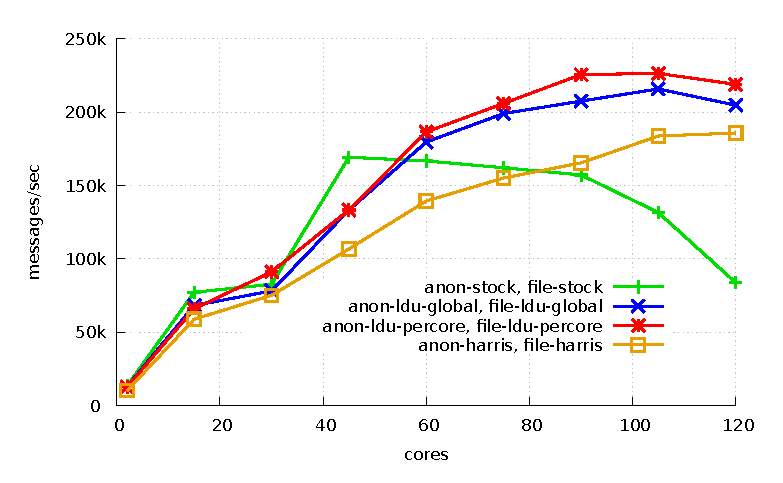
\includegraphics[scale=0.65]{graph/exim.eps}
  \end{center}
  \caption{Scalability of Exim. The stock Linux collapses after 60 core;in
  contrast, both unordered harris list and our \deferu flatten out.}
  \label{fig:exim}
\end{figure}
\subsection{Exim}
%$$$$$$$$$$$$$$$$$$$$$$$$$$$$$$$$$$$$$$$$$$$$$$$$$$$$$$$$$$$$$$$$$$$$$$$$$$$$$$$$
%Paragraph 1:  EXIM 실험 결과
%$$$$$$$$$$$$$$$$$$$$$$$$$$$$$$$$$$$$$$$$$$$$$$$$$$$$$$$$$$$$$$$$$$$$$$$$$$$$$$$$

\begin{figure}[tb]
  \begin{center}
    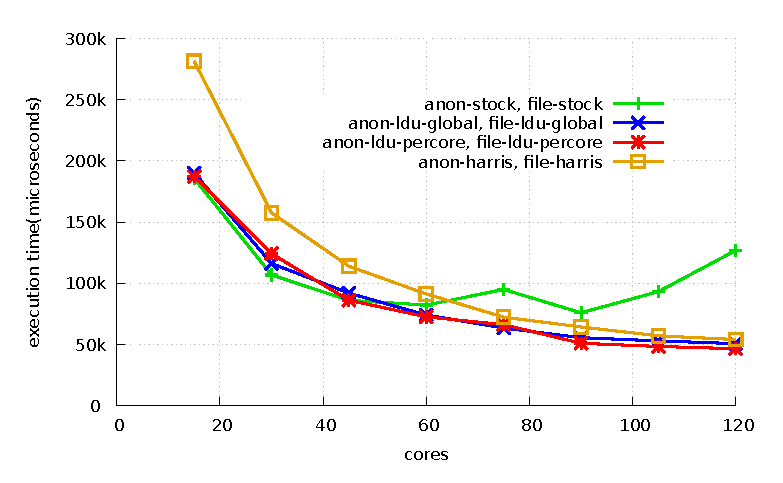
\includegraphics[scale=0.65]{graph/lmbench.eps}
  \end{center}
  \caption{Execution time of lmbench's fork micro benchmark. The fork micro
  benchmark drops down for all methods up to 15 core but either flattens out or
  goes up slightly after that. At 15 core, the stock Linux goes up;the others
  flattens out}
  \label{fig:MicroBench}
\end{figure}



%$$$$$$$$$$$$$$$$$$$$$$$$$$$$$$$$$$$$$$$$$$$$$$$$$$$$$$$$$$$$$$$$$$$$$$$$$$$$$$$$
%Paragraph 1: 워크로드에 대한 설명
%$$$$$$$$$$$$$$$$$$$$$$$$$$$$$$$$$$$$$$$$$$$$$$$$$$$$$$$$$$$$$$$$$$$$$$$$$$$$$$$$
To measure the performance of Exim, shown in Figure~\ref{fig:exim}, we
used default value of MOSBENCH to use tmpfs for
spool files, log files, and user mail files.
Clients run on the same machine and each client sends to a different user to
prevent contention on user mail file.
The Exim was bottlenecked by per-directory locks protecting file creation in
the spool directories and by forks performed on different
cores~\cite{SilasBoydWickizer2010LinuxScales48}.
Therefore, although we eliminate the fork problem, the Exim may suffer from
contention on spool directories. 

%$$$$$$$$$$$$$$$$$$$$$$$$$$$$$$$$$$$$$$$$$$$$$$$$$$$$$$$$$$$$$$$$$$$$$$$$$$$$$$$$
%Paragraph 2:실험 결과에 대한 설명
%$$$$$$$$$$$$$$$$$$$$$$$$$$$$$$$$$$$$$$$$$$$$$$$$$$$$$$$$$$$$$$$$$$$$$$$$$$$$$$$$
Results shown in Figure~\ref{fig:exim} show that Exim scales well for all
methods up to 60 core but not for higher core counts.
The stock Linux shows performance degradation for more than 60 core.
Both unordered harris list
and our \deferu do not suffer from performance loss 
because they do not acquire the \code{anon\_vma}
semaphore and \code{i\_mmap} semaphore in fork.
\deferu performs better due to the fact that it uses both update-side
absorbing and lock-less list, outperforming stock Linux by 1.6x and unordered
harris list by 1.1x.
Even though we applied scalable solution, Exim shows limitation on scalability
improvement
since the main bottleneck is per-directory lock contention on spool
directories.
The unordered harris list has 31\% idle time, whereas \deferu has 37\% idle
time due to the their efficient concurrent updates.

\begin{figure*}[t!]
    \centering
    \begin{subfigure}[b]{0.33\textwidth}
        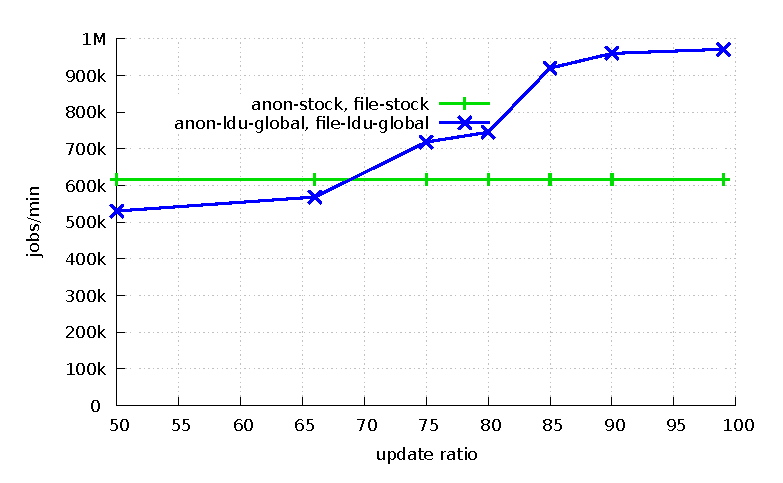
\includegraphics[height=1.3in]{graph/ratio_aim7.eps}
        \caption{AIM7 - 120core}
    \end{subfigure}%
    \begin{subfigure}[b]{0.33\textwidth}
        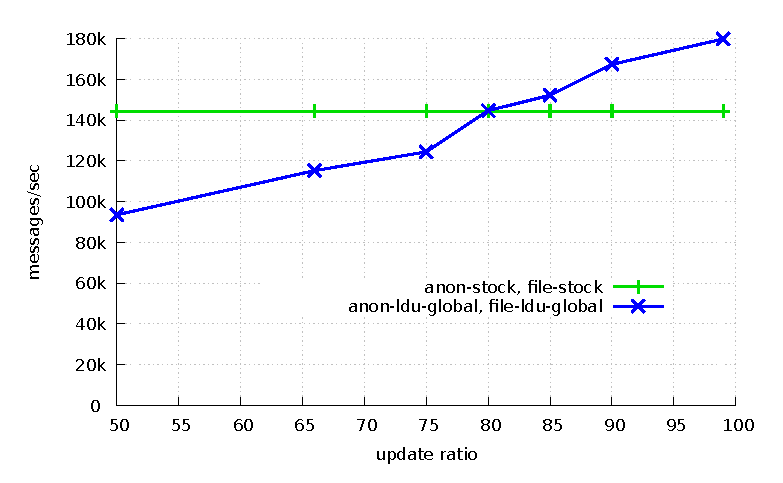
\includegraphics[height=1.3in]{graph/ratio_exim.eps}
        \caption{Exim - 120core}
    \end{subfigure}
    \begin{subfigure}[b]{0.33\textwidth}
        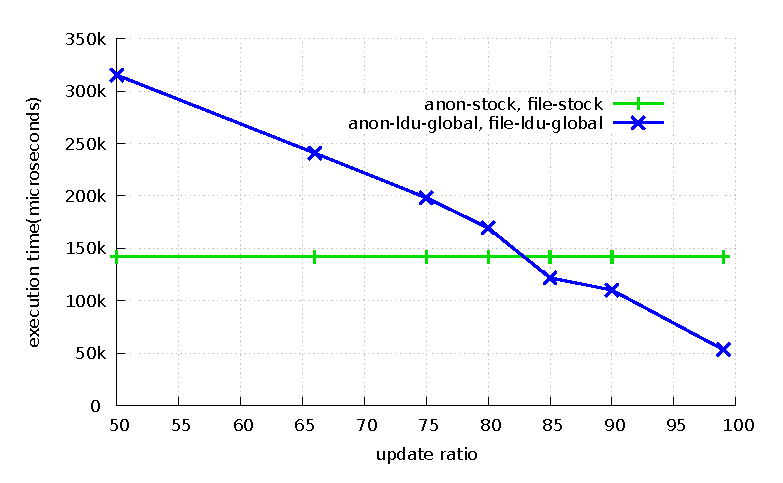
\includegraphics[height=1.3in]{graph/ratio_lmbench.eps}
        \caption{Lmbench - 120core}
    \end{subfigure}
        \centering
    \begin{subfigure}[b]{0.33\textwidth}
        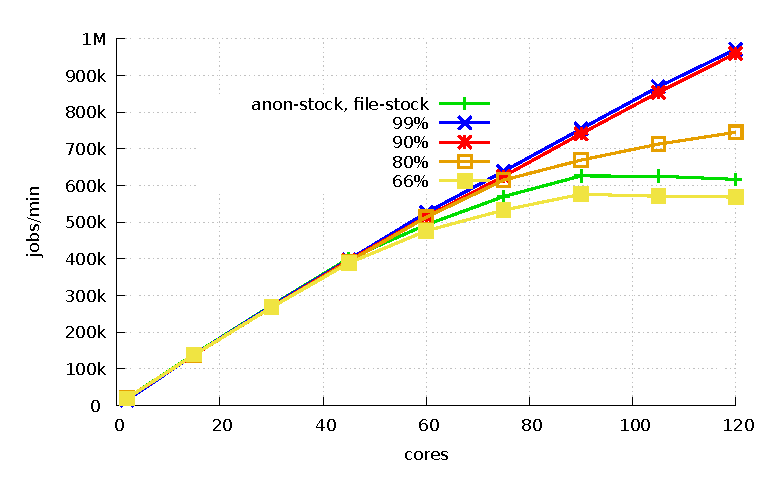
\includegraphics[height=1.3in]{graph/ratio_aim7_core.eps}
        \caption{AIM7 - scalability}
    \end{subfigure}%
    \begin{subfigure}[b]{0.33\textwidth}
        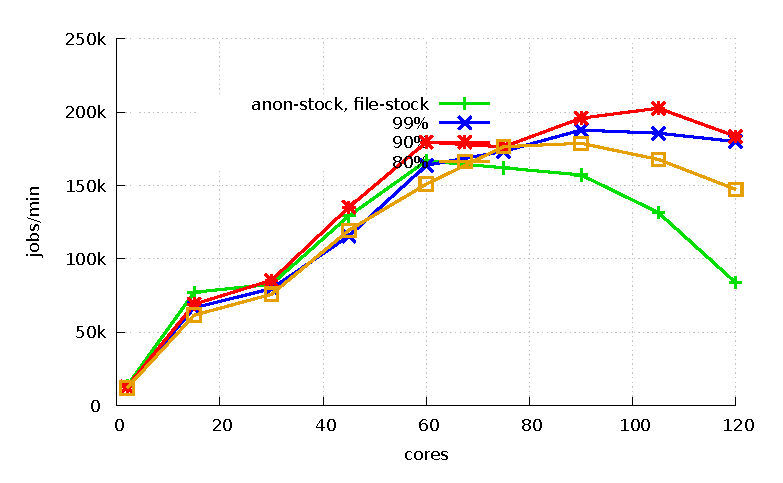
\includegraphics[height=1.3in]{graph/ratio_exim_core.eps}
        \caption{Exim - scalability}
    \end{subfigure}
    \begin{subfigure}[b]{0.33\textwidth}
        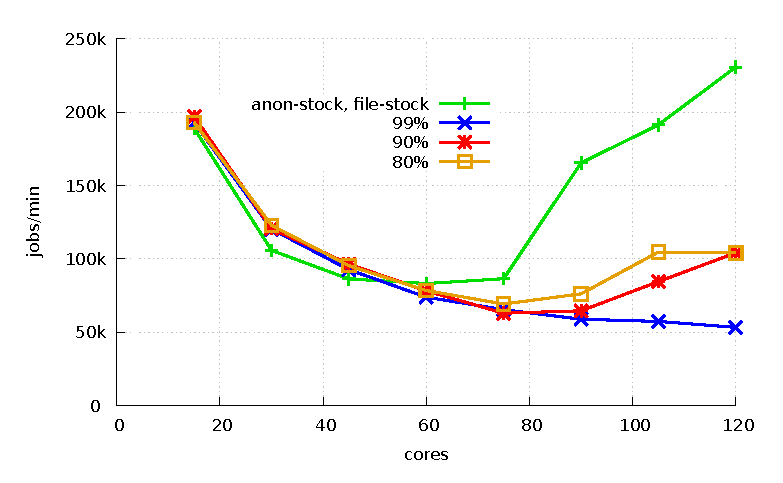
\includegraphics[height=1.3in]{graph/ratio_lmbench_core.eps}
        \caption{Lmbench - scalability}
    \end{subfigure}
    \caption{Read-write ratio from 50:50 to 1:99 percent}
    
\end{figure*}

\subsection{Lmbench}
%$$$$$$$$$$$$$$$$$$$$$$$$$$$$$$$$$$$$$$$$$$$$$$$$$$$$$$$$$$$$$$$$$$$$$$$$$$$$$$$$
%Paragraph 1: %워크로드에 대한 설명
%$$$$$$$$$$$$$$$$$$$$$$$$$$$$$$$$$$$$$$$$$$$$$$$$$$$$$$$$$$$$$$$$$$$$$$$$$$$$$$$$
lmbench has various workloads including process creation workload(fork,
exec, sh -c, exit).
This workload is used to measure the basic process primitives such as creating
a new process, running a different program, and context switching. 
We configured process create workload to enable the parallelism option which
specifies the number of benchmark processes to run in
parallel~\cite{mcvoy1996lmbench}; we used 100 processes.

%$$$$$$$$$$$$$$$$$$$$$$$$$$$$$$$$$$$$$$$$$$$$$$$$$$$$$$$$$$$$$$$$$$$$$$$$$$$$$$$$
%Paragraph 2: 실험 결과에 대한 설명
%$$$$$$$$$$$$$$$$$$$$$$$$$$$$$$$$$$$$$$$$$$$$$$$$$$$$$$$$$$$$$$$$$$$$$$$$$$$$$$$$
The results for lmbench are shown in Figure~\ref{fig:MicroBench}, 
and the results show the execution times of the fork microbenchmark in lmbench
with four different methods.
%The fork micro benchmark drops down for all methods up to 15 core but either
%flattens out or goes up slightly after that.
Three methods outperform stock Linux by 2.2x at 120 cores;however, before 30
core, two harris list have lower performance due to their execution overheads.
%At 15 core, the stock Linux goes up because of the NUMA effect that accesses
%the remote memory.
%On the other hand, the others including the ordered harris list flattens out
%and then they remain constant.
While stock Linux has 90\% idle time, other methods have approximately 50\%
idle time since stock Linux waits to acquire reverse mapping locks such as
\code{anon\_vma's rwsem} and \code{mapping's i\_mmap\_rwsem}.




\subsection{Updates ratio}



%$$$$$$$$$$$$$$$$$$$$$$$$$$$$$$$$$$$$$$$$$$$$$$$$$$$$$$$$$$$$$$$$$$$$$$$$$$$$$$$$
%Paragraph 2:  실험을 수행한 이유
%$$$$$$$$$$$$$$$$$$$$$$$$$$$$$$$$$$$$$$$$$$$$$$$$$$$$$$$$$$$$$$$$$$$$$$$$$$$$$$$$
The LDU is a method for update-heavy data structure.
That is, the LDU can show substantial scalability where the data structures are
frequently updates but rarely read because the read operation executes the
synchronize function to apply logs.
That means the read operations can be slower.
To further evaluate LDU and to understand the effect of read operation, we
perform the additional read operation with respect to the rmap.
The anonymous rmap uses the version of ldu with global queue because we
merely focus on read ratio and then we sequentially increase read (lock and
synchronize) ratios regarding the file rmap.
%$$$$$$$$$$$$$$$$$$$$$$$$$$$$$$$$$$$$$$$$$$$$$$$$$$$$$$$$$$$$$$$$$$$$$$$$$$$$$$$$
%Paragraph 2: 실험 결과에 대한 설명
%$$$$$$$$$$$$$$$$$$$$$$$$$$$$$$$$$$$$$$$$$$$$$$$$$$$$$$$$$$$$$$$$$$$$$$$$$$$$$$$$
The upper graphs of Figure x-x  shows the performance on 120 core depending
on read rate, and the lower graphs represent the scalability.
Since the AIM7 has less fork-intensive workload feature than other ones, the
read operations are invoked relatively infrequently.
As a result, although the data structure uses 75 percent(3
update, 1 read) update rate, the AIM7 has outstanding performance than stock
Linux.
The scalability of AIM7 shows that LDU substantially high scalability at the
over the 90 percent update rate, and 80 percent update rates slightly. 

The result of the Exim and the Lmbench shows the more high fork-intensive
workload represents the read operations high effects

